% $Id: ESMF_superoverview.tex,v 1.10 2004/03/24 20:01:00 cdeluca Exp $
%
% Earth System Modeling Framework
% Copyright 2002-2003, University Corporation for Atmospheric Research, 
% Massachusetts Institute of Technology, Geophysical Fluid Dynamics 
% Laboratory, University of Michigan, National Centers for Environmental 
% Prediction, Los Alamos National Laboratory, Argonne National Laboratory, 
% NASA Goddard Space Flight Center.
% Licensed under the GPL.

\section{Overview of Superstructure}

The ESMF superstructure classes define an architecture for assembling
Earth system applications from modeling components.  Earth system research 
often requires that large scale components such as atmosphere, ocean,
and land models be coupled together to create an application.  
Coupling components may involve both data transformations and, on 
parallel computing systems, data transfers.  The ESMF offers coupling 
services to simplify the organization and execution of inter-component 
data exchange.  ESMF coupling services can also be utilized for 
smaller-scale tasks within components, such as the 
transformation of data between the physics and dynamics in a spectral 
atmosphere model, or the creation of nested higher resolution regions 
within a coarser grid.  The objective is to couple components at varying 
scales both flexibly and efficiently.  The ESMF encourages a hierachical
application structure, in which large components branch into 
smaller sub-components.  It also allows the same component to be 
used in multiple contexts without changes to its source code.

\begin{center}  
\begin{tabular}{|p{6in}|}
\hline
\vspace{.01in}
{\bf Key Features} \\[.01in]
Modular, component-based architecture. \\
Hierarchical assembly of components into applications.\\
Use of components in multiple contexts without modification.\\
Sequential or concurrent component execution.\\
Single program, multiple datastream (SPMD) applications for 
maximum portability and reconfigurability.\\[.03in] \hline
\end{tabular}
\end{center}

\subsection{Superstructure Classes}

There are a small number of classes in the ESMF superstructure:

\begin{itemize}
\item {\bf Component}  An ESMF component has two parts, one that is 
supplied by the ESMF and one that is supplied by the user.  The
part that is supplied by the framework is an ESMF derived type that
is either a Gridded Component ({\bf GridComp}) or a Coupler 
Component ({\bf CplComp}).  A Gridded Component typically represents
a physical domain in which data is associated with one or more 
grids - for example, a sea ice model.  A Coupler Component 
arranges and executes data transformations and transfers between 
one or more Gridded Components. Gridded Components and Coupler 
Components have standard methods, which include Run, Initialize,
and Finalize.  These methods can be multi-phase.

The second part of an ESMF Component is user code, such as a
model or data assimilation system.  Users register their code with 
the framework in order to make it part of an ESMF application.  
In practice, registration means that within the user-written 
software there are calls to ESMF methods that associate a 
standard ESMF operation with the name of the corresponding 
Fortran subroutine in their user code.  For example, a user-written
initialization routine called {\tt popOceanInit} might be 
associated with the standard Initialize routine of an ESMF 
Gridded Component named ``POP'' that represents an ocean model.

\item {\bf State}  ESMF components exchange information with other 
components only through States.  A State is an ESMF derived
type that can contain Fields, Bundles, Arrays, and other
States.  A Gridded Component  is associated with two States, an 
{\bf Import State} and an {\bf Export State}.  Its Import State 
holds the data that it receives from other Gridded Components.  
Its Export State contains data that it can make available to 
other Gridded Components. 

\item {\bf Application Driver} The Application Driver ({\bf AppDriver}) 
is a small, generic driver program that contains the ``main'' 
routine for an ESMF application.

\end{itemize}

An ESMF coupled application typically involves an AppDriver, a parent 
Gridded Component, two or more child Gridded Components that require 
an inter-component data exchange, and one or more Coupler 
Components. 

The parent Gridded Component is responsible for creating the child 
Gridded Components that are exchanging data and creating the Coupler, 
for creating the necessary Import and Export States, and for 
setting up the desired sequencing.  The AppDriver ``main'' routine
calls the parent Gridded Component's Initialize, Run, and Finalize 
methods in order to execute the application.  For each of these
standard methods, the parent Gridded Component in turn calls the 
corresponding methods in the child Gridded Components and the 
Coupler Component.  For example, consider a simple coupled 
ocean/atmosphere simulation.  When the Initialize method of the 
parent Gridded Component is called by the AppDriver, it in turn 
calls the Initialize methods of its child atmosphere and ocean 
Gridded Components, and the Initialize method of an 
ocean-to-atmosphere Coupler Component.

The framework supplies methods to do basic transformations which 
may include regridding, interpolation, unit conversions, 
accumulations, averaging, transformations which conserve specific 
values.

\subsection{Distribution and Scoping of Components}
\label{sec:scoping}

Components are distributed across Distribution Elements, or {\bf DEs}.
A DE represents a piece of a decomposition.  A DELayout is a collection
of DEs with some associated connectivity that describes a specific 
distribution.  For example, the distribution of a grid divided 
into four segments in the x-dimension would be expressed in ESMF as
a DELayout with four DEs lying along an x-axis. On parallel computing
systems, a DE is often associated with a distinct computational resource, 
such as a processor or a Posix thread.  

All data transfers within an ESMF application occur {\it within} a 
component.  For example, a Gridded Component may contain halo updates.
Another example is that a Coupler Component may contain a regridding 
and data redistribution between two Gridded Components.  As a result, 
the architecture of ESMF does not depend on any particular data 
communication mechanism, and new communication schemes can be 
introduced without affecting the overall structure of the application.

Since all data communication happens within a component, a Coupler 
Component must be created on the union of the DEs of all
the Gridded Components it couples.  

A Gridded Component may exist across all the DEs in an application.  
A Gridded Component may also reside on a subset of DEs in an 
application.  These DEs may wholly coincide with, be wholly contained 
within, or wholly contain another component.  

When a set of Gridded  Components and a Coupler runs in sequence 
on the same set of DEs the application is executing in a {\bf sequential} 
mode. When Gridded Components are created and run on mutually exclusive
sets of DEs, and are coupled by a Coupler Component that extends over
the union of these sets, the mode of execution is {\bf concurrent}.

It is possible for ESMF applications to contain some component sets
that are executing sequentially and others that are executing concurrently.
We might have, for example, atmosphere and land components created 
on the same subset of DEs, ocean and sea ice components created on 
the remainder of DEs, and a Coupler created across all the DEs in
the application.

\subsection{Performance}
\label{sec:performance}

The ESMF design enables the user to configure ESMF
applications so that data is transferred from one component to another, 
without requiring that it be copied or sent to a different data
buffers as interim steps.  This is likely to be the most efficient way 
of performing inter-component coupling when the components are instantiated 
on different DE sets.  However, if desired, an application can also be 
configured so that data from a source component is sent to a distinct set of 
Coupler Component DEs for processing before being sent to its 
destination.

The ability to overlap computation with communication is essential for
performance.  When running with ESMF the user can initiate data 
sends during Gridded Component execution, as soon as the data is ready.
The computation can then proceed simultaneously with the data transfer.

\newpage
\subsection{Object Model}

The following is a simplified UML diagram showing the relationships among
ESMF superstructure classes.  See Appendix A, {\it A Brief 
Introduction to UML},
for a translation table that lists the symbols in the diagram and their 
meaning.

\begin{center}
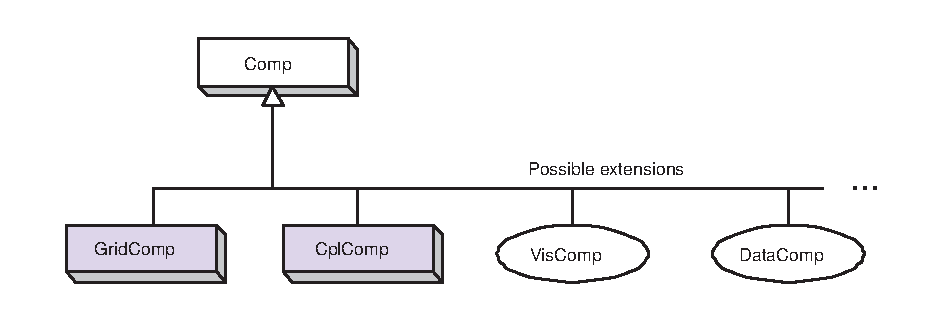
\includegraphics{Comp_obj.eps}   
\end{center}



